\section{Результаты}
\subsection{Гистограмма и график плотности распределения}
\begin{figure}[H]
	\center{\includegraphics[width=1\linewidth]{task1\_images/Norm}}
	\caption{ Нормальное распределение.}
	\label{ris:1}
\end{figure}
\begin{figure}[H]
	\center{\includegraphics[width=1\linewidth]{task1\_images/Cauchy}}
	\caption{ Распределение Коши.}
	\label{ris:2}
\end{figure}
\begin{figure}[H]
	\center{\includegraphics[width=1\linewidth]{task1\_images/Laplace}}
	\caption{ Распределение Лапласа.}
	\label{ris:3}
\end{figure}
\begin{figure}[H]
	\center{\includegraphics[width=1\linewidth]{task1\_images/Poisson}}
	\caption{ Распределение Пуассона.}
	\label{ris:4}
\end{figure}
\begin{figure}[H]
	\center{\includegraphics[width=1\linewidth]{task1\_images/Uniform}}
	\caption{ Равномерное распределение.}
	\label{ris:5}
\end{figure}

\subsection{Характеристики положения и рассеяния}
\begin{table}[H]
	\begin{center}
		\begin{tabular}{|c|c|c|c|c|c|}
\hline
 & $\bar{x} \, (\ref{8})$ & $med \, x \, (\ref{9})$ & $z_R \, (\ref{10})$ & $z_Q \, (\ref{12})$ & $z_{tr} \, (\ref{13})$ \\
\hline
n =10 &  &  &  &  & \\
\hline
$E(z) \, (\ref{1})$ & -0.0037 & 0.0062 & 0.005 & 0.3029 & 0.1099\\
\hline
$D(z) \, (\ref{2})$ & 0.1052 & 0.1444 & 0.1893 & 0.1312 & 0.0846\\
\hline
$E(z)+sqrt(D(z))$ & 0.3206 & 0.3861 & 0.4401 & 0.6652 & 0.4008\\
\hline
$E(z)-sqrt(D(z))$ & -0.328 & -0.3738 & -0.4301 & -0.0593 & -0.181\\
\hline
$\hat{E(z)}$ & 0 & 0 & 0 & 0 & 0\\
\hline
n =100 &  &  &  &  & \\
\hline
$E(z) \, (\ref{1})$ & -0.001 & -0.0001 & -0.0042 & 0.0156 & 0.0129\\
\hline
$D(z) \, (\ref{2})$ & 0.0099 & 0.015 & 0.0911 & 0.0121 & 0.0114\\
\hline
$E(z)+sqrt(D(z))$ & 0.0983 & 0.1224 & 0.2976 & 0.1255 & 0.1194\\
\hline
$E(z)-sqrt(D(z))$ & -0.1004 & -0.1225 & -0.306 & -0.0942 & -0.0937\\
\hline
$\hat{E(z)}$ & 0 & 0 & 0 & 0 & 0\\
\hline
n =1000 &  &  &  &  & \\
\hline
$E(z) \, (\ref{1})$ & -0.0002 & -0.0003 & 0.0092 & 0.0012 & 0.0011\\
\hline
$D(z) \, (\ref{2})$ & 0.001 & 0.0015 & 0.0597 & 0.0013 & 0.0012\\
\hline
$E(z)+sqrt(D(z))$ & 0.0316 & 0.0385 & 0.2535 & 0.0367 & 0.0353\\
\hline
$E(z)-sqrt(D(z))$ & -0.032 & -0.0391 & -0.2351 & -0.0342 & -0.0332\\
\hline
$\hat{E(z)}$ & 0 & 0 & 0 & 0 & 0\\
\hline
\end{tabular}
	\end{center}
	\caption{\label{tab:2} Нормальное распределение.}
\end{table}
\begin{table}[H]
	\begin{center}
		\begin{tabular}{|c|c|c|c|c|c|}
\hline
 & $\bar{x} \, (\ref{8})$ & $med \, x \, (\ref{9})$ & $z_R \, (\ref{10})$ & $z_Q \, (\ref{12})$ & $z_{tr} \, (\ref{13})$ \\
\hline
n =10 &  &  &  &  & \\
\hline
$E(z) \, (\ref{1})$ & -0.608 & -0.0563 & -2.6781 & 1.0598 & 0.15\\
\hline
$D(z) \, (\ref{2})$ & 207.6975 & 0.3392 & 5098.0099 & 5.0939 & 0.3125\\
\hline
$E(z)+sqrt(D(z))$ & 13.8037 & 0.5261 & 68.7222 & 3.3168 & 0.7091\\
\hline
$E(z)-sqrt(D(z))$ & -15.0198 & -0.6387 & -74.0785 & -1.1972 & -0.409\\
\hline
$\hat{E(z)}$ & - & 0 & - & - & 0\\
\hline
n =100 &  &  &  &  & \\
\hline
$E(z) \, (\ref{1})$ & 4.9756 & -0.0064 & 250.1532 & 0.0229 & 0.012\\
\hline
$D(z) \, (\ref{2})$ & 30895.3926 & 0.0246 & 77201763.7001 & 0.0527 & 0.0249\\
\hline
$E(z)+sqrt(D(z))$ & 180.7464 & 0.1504 & 9036.6066 & 0.2524 & 0.1697\\
\hline
$E(z)-sqrt(D(z))$ & -170.7953 & -0.1631 & -8536.3002 & -0.2066 & -0.1457\\
\hline
$\hat{E(z)}$ & - & 0 & - & 0 & 0\\
\hline
n =1000 &  &  &  &  & \\
\hline
$E(z) \, (\ref{1})$ & 148.5074 & 0.0009 & 74233.3648 & 0.0036 & 0.0026\\
\hline
$D(z) \, (\ref{2})$ & 21792325.6629 & 0.0024 & 5448026807934.155 & 0.0047 & 0.0025\\
\hline
$E(z)+sqrt(D(z))$ & 4816.7325 & 0.0503 & 2408334.2212 & 0.0723 & 0.0528\\
\hline
$E(z)-sqrt(D(z))$ & -4519.7177 & -0.0484 & -2259867.4917 & -0.0651 & -0.0476\\
\hline
$\hat{E(z)}$ & - & 0.0 & - & 0.0 & 0.0\\
\hline
\end{tabular}
	\end{center}
	\caption{\label{tab:3} Распределение Коши.}
\end{table}
\begin{table}[H]
	\begin{center}
		\begin{tabular}{|c|c|c|c|c|c|}
\hline
 & $\bar{x} \, (\ref{8})$ & $med \, x \, (\ref{9})$ & $z_R \, (\ref{10})$ & $z_Q \, (\ref{12})$ & $z_{tr} \, (\ref{13})$ \\
\hline
n =10 &  &  &  &  & \\
\hline
$E(z) \, (\ref{1})$ & 0.0039 & -0.0074 & 0.0251 & 0.2928 & 0.0836\\
\hline
$D(z) \, (\ref{2})$ & 0.0913 & 0.0701 & 0.3548 & 0.1135 & 0.0481\\
\hline
$E(z)+sqrt(D(z))$ & 0.306 & 0.2573 & 0.6207 & 0.6297 & 0.3029\\
\hline
$E(z)-sqrt(D(z))$ & -0.2982 & -0.2722 & -0.5705 & -0.044 & -0.1357\\
\hline
$\hat{E(z)}$ & 0 & 0 & 0 & 0 & 0\\
\hline
n =100 &  &  &  &  & \\
\hline
$E(z) \, (\ref{1})$ & -0.004 & -0.0025 & -0.0097 & 0.0122 & 0.0077\\
\hline
$D(z) \, (\ref{2})$ & 0.0097 & 0.0055 & 0.4056 & 0.0092 & 0.0056\\
\hline
$E(z)+sqrt(D(z))$ & 0.0946 & 0.0714 & 0.6272 & 0.108 & 0.0825\\
\hline
$E(z)-sqrt(D(z))$ & -0.1026 & -0.0763 & -0.6466 & -0.0836 & -0.0671\\
\hline
$\hat{E(z)}$ & 0 & 0 & 0 & 0 & 0\\
\hline
n =1000 &  &  &  &  & \\
\hline
$E(z) \, (\ref{1})$ & 0.0 & -0.0001 & 0.0016 & 0.0015 & 0.0012\\
\hline
$D(z) \, (\ref{2})$ & 0.001 & 0.0005 & 0.4074 & 0.001 & 0.0006\\
\hline
$E(z)+sqrt(D(z))$ & 0.0314 & 0.0227 & 0.6399 & 0.0334 & 0.026\\
\hline
$E(z)-sqrt(D(z))$ & -0.0313 & -0.0229 & -0.6367 & -0.0305 & -0.0235\\
\hline
$\hat{E(z)}$ & 0 & 0 & 0 & 0 & 0\\
\hline
\end{tabular}
	\end{center}
	\caption{\label{tab:4} Распределение Лапласа.}
\end{table}
\begin{table}[H]
	\begin{center}
		\begin{tabular}{|c|c|c|c|c|c|}
\hline
 & $\bar{x} \, (\ref{8})$ & $med \, x \, (\ref{9})$ & $z_R \, (\ref{10})$ & $z_Q \, (\ref{12})$ & $z_{tr} \, (\ref{13})$ \\
\hline
n =10 &  &  &  &  & \\
\hline
$E(z) \, (\ref{1})$ & 9.9588 & 9.8375 & 10.233 & 10.9165 & 8.5568\\
\hline
$D(z) \, (\ref{2})$ & 1.0631 & 1.4818 & 2.0712 & 1.4253 & 0.89\\
\hline
$E(z)+sqrt(D(z))$ & 10.9899 & 11.0548 & 11.6722 & 12.1103 & 9.5002\\
\hline
$E(z)-sqrt(D(z))$ & 8.9277 & 8.6202 & 8.7938 & 9.7227 & 7.6135\\
\hline
$\hat{E(z)}$ & 10 & 10 & 10 & 10 & 10\\
\hline
n =100 &  &  &  &  & \\
\hline
$E(z) \, (\ref{1})$ & 9.9989 & 9.846 & 10.9275 & 9.981 & 9.7031\\
\hline
$D(z) \, (\ref{2})$ & 0.1086 & 0.2218 & 0.8995 & 0.1641 & 0.1227\\
\hline
$E(z)+sqrt(D(z))$ & 10.3284 & 10.3169 & 11.8759 & 10.3861 & 10.0533\\
\hline
$E(z)-sqrt(D(z))$ & 9.6694 & 9.3751 & 9.9791 & 9.5759 & 9.3528\\
\hline
$\hat{E(z)}$ & 10 & 10 & 10 & 10 & 10\\
\hline
n =1000 &  &  &  &  & \\
\hline
$E(z) \, (\ref{1})$ & 9.9967 & 9.9965 & 11.6625 & 9.9935 & 9.8393\\
\hline
$D(z) \, (\ref{2})$ & 0.0109 & 0.0032 & 0.7058 & 0.0032 & 0.0116\\
\hline
$E(z)+sqrt(D(z))$ & 10.1008 & 10.0534 & 12.5026 & 10.0501 & 9.9471\\
\hline
$E(z)-sqrt(D(z))$ & 9.8925 & 9.9396 & 10.8224 & 9.9369 & 9.7315\\
\hline
$\hat{E(z)}$ & 10 & 10 & 10 & 10 & 10\\
\hline
\end{tabular}
	\end{center}
	\caption{\label{tab:5} Распределение Пуассона.}
\end{table}
\begin{table}[H]
	\begin{center}
		\begin{tabular}{|c|c|c|c|c|c|}
\hline
 & $\bar{x} \, (\ref{8})$ & $med \, x \, (\ref{9})$ & $z_R \, (\ref{10})$ & $z_Q \, (\ref{12})$ & $z_{tr} \, (\ref{13})$ \\
\hline
n =10 &  &  &  &  & \\
\hline
$E(z) \, (\ref{1})$ & -0.0026 & 0.0001 & -0.0033 & 0.3074 & 0.1302\\
\hline
$D(z) \, (\ref{2})$ & 0.103 & 0.2303 & 0.0493 & 0.1319 & 0.1235\\
\hline
$E(z)+sqrt(D(z))$ & 0.3183 & 0.48 & 0.2188 & 0.6706 & 0.4816\\
\hline
$E(z)-sqrt(D(z))$ & -0.3235 & -0.4798 & -0.2254 & -0.0559 & -0.2212\\
\hline
$\hat{E(z)}$ & 0 & 0 & 0 & 0 & 0\\
\hline
n =100 &  &  &  &  & \\
\hline
$E(z) \, (\ref{1})$ & -0.0017 & -0.0086 & -0.0007 & 0.0162 & 0.0134\\
\hline
$D(z) \, (\ref{2})$ & 0.0101 & 0.0294 & 0.0006 & 0.015 & 0.0192\\
\hline
$E(z)+sqrt(D(z))$ & 0.0986 & 0.1628 & 0.0235 & 0.1386 & 0.1519\\
\hline
$E(z)-sqrt(D(z))$ & -0.102 & -0.1799 & -0.0248 & -0.1062 & -0.1251\\
\hline
$\hat{E(z)}$ & 0 & 0 & 0.0 & 0 & 0\\
\hline
n =1000 &  &  &  &  & \\
\hline
$E(z) \, (\ref{1})$ & 0.0011 & 0.0013 & 0.0001 & 0.0037 & 0.0029\\
\hline
$D(z) \, (\ref{2})$ & 0.001 & 0.0031 & 0.0 & 0.0015 & 0.0021\\
\hline
$E(z)+sqrt(D(z))$ & 0.0335 & 0.0566 & 0.0025 & 0.043 & 0.0484\\
\hline
$E(z)-sqrt(D(z))$ & -0.0312 & -0.054 & -0.0024 & -0.0357 & -0.0426\\
\hline
$\hat{E(z)}$ & 0.0 & 0.0 & 0.0 & 0.0 & 0.0\\
\hline
\end{tabular}
	\end{center}
	\caption{\label{tab:6} Равномерное распределение.}
\end{table}

\subsection{Боксплот Тьюки}
\begin{figure}[H]
	\center{\includegraphics[width=0.65\linewidth]{task3\_data/Norm}}
	\caption{ Нормальное распределение.}
	\label{ris:6}
\end{figure}
\begin{figure}[H]
	\center{\includegraphics[width=0.65\linewidth]{task3\_data/Cauchy}}
	\caption{ Распределение Коши.}
	\label{ris:7}
\end{figure}
\begin{figure}[H]
	\center{\includegraphics[width=0.65\linewidth]{task3\_data/Laplace}}
	\caption{ Распределение Лапласа.}
	\label{ris:8}
\end{figure}
\begin{figure}[H]
	\center{\includegraphics[width=0.65\linewidth]{task3\_data/Poisson}}
	\caption{ Распределение Пуассона.}
	\label{ris:9}
\end{figure}
\begin{figure}[H]
	\center{\includegraphics[width=0.65\linewidth]{task3\_data/Uniform}}
	\caption{ Равномерное распределение.}
	\label{ris:10}
\end{figure}

\subsection{Доля выбросов}
\begin{table}[H]
	\begin{center}
		\begin{tabular}{|c|c|}
\hline
Sample & Share of emissions \\
\hline
Norm n = $20$ & $0.023$\\
\hline
Norm n = $100$ & $0.01$\\
\hline
Cauchy n = $20$ & $0.151$\\
\hline
Cauchy n = $100$ & $0.155$\\
\hline
Laplace n = $20$ & $0.072$\\
\hline
Laplace n = $100$ & $0.067$\\
\hline
Poisson n = $20$ & $0.024$\\
\hline
Poisson n = $100$ & $0.01$\\
\hline
Uniform n = $20$ & $0.002$\\
\hline
Uniform n = $100$ & $0.0$\\
\hline
\end{tabular}
	\end{center}
	\caption{\label{tab:7} Экспериментальная доля выбросов.}
\end{table}

\subsection{Теоретическая вероятность выбросов}
\begin{table}[H]
	\begin{center}
		\begin{tabular}{|c|c|}
			\hline
			Распределение & $P_B^T \,(\ref{17}),(\ref{18})$ \\
			\hline
			Нормальное распределение & 0.007\\
			\hline
			Распределение Коши  & 0.156\\
			\hline
			Распределение Лапласа & 0.063\\
			\hline
			Распределение Пуассона & 0.008\\
			\hline
			Равномерное распределение & 0\\
			\hline
		\end{tabular}
	\end{center}
	\caption{\label{tab:8} Теоретическая вероятность выбросов.}
\end{table}

\subsection{Эмпирическая функция распределения}
\begin{figure}[H]
	\center{\includegraphics[width=1\linewidth]{task4\_data/Norm\_emperic\_f}}
	\caption{ Нормальное распределение.}
	\label{ris:11}
\end{figure}
\begin{figure}[H]
	\center{\includegraphics[width=1\linewidth]{task4\_data/Cauchy\_emperic\_f}}
	\caption{ Распределение Коши.}
	\label{ris:12}
\end{figure}
\begin{figure}[H]
	\center{\includegraphics[width=1\linewidth]{task4\_data/Laplace\_emperic\_f}}
	\caption{ Распределение Лапласа.}
	\label{ris:13}
\end{figure}
\begin{figure}[H]
	\center{\includegraphics[width=1\linewidth]{task4\_data/Poisson\_emperic\_f}}
	\caption{ Распределение Пуассона.}
	\label{ris:14}
\end{figure}
\begin{figure}[H]
	\center{\includegraphics[width=1\linewidth]{task4\_data/Uniform\_emperic\_f}}
	\caption{ Равномерное распределение.}
	\label{ris:15}
\end{figure}

\subsection{Ядерные оценки плотности распределения}
\begin{figure}[H]
	\center{\includegraphics[width=1\linewidth]{task4\_data/Norm\_kernel\_n20}}
	\caption{ Нормальное распределение n = 20.}
	\label{ris:16}
\end{figure}
\begin{figure}[H]
	\center{\includegraphics[width=1\linewidth]{task4\_data/Norm\_kernel\_n60}}
	\caption{ Нормальное распределение n = 60.}
	\label{ris:17}
\end{figure}
\begin{figure}[H]
	\center{\includegraphics[width=1\linewidth]{task4\_data/Norm\_kernel\_n100}}
	\caption{ Нормальное распределение n = 100.}
	\label{ris:18}
\end{figure}
\begin{figure}[H]
	\center{\includegraphics[width=1\linewidth]{task4\_data/Cauchy\_kernel\_n20}}
	\caption{ Распределение Коши n = 20.}
	\label{ris:19}
\end{figure}
\begin{figure}[H]
	\center{\includegraphics[width=1\linewidth]{task4\_data/Cauchy\_kernel\_n60}}
	\caption{ Распределение Коши n = 60.}
	\label{ris:20}
\end{figure}
\begin{figure}[H]
	\center{\includegraphics[width=1\linewidth]{task4\_data/Cauchy\_kernel\_n100}}
	\caption{ Распределение Коши n = 100.}
	\label{ris:21}
\end{figure}
\begin{figure}[H]
	\center{\includegraphics[width=1\linewidth]{task4\_data/Laplace\_kernel\_n20}}
	\caption{ Распределение Лапласа n = 20.}
	\label{ris:22}
\end{figure}
\begin{figure}[H]
	\center{\includegraphics[width=1\linewidth]{task4\_data/Laplace\_kernel\_n60}}
	\caption{ Распределение Лапласа n = 60.}
	\label{ris:23}
\end{figure}
\begin{figure}[H]
	\center{\includegraphics[width=1\linewidth]{task4\_data/Laplace\_kernel\_n100}}
	\caption{ Распределение Лапласа n = 100.}
	\label{ris:24}
\end{figure}
\begin{figure}[H]
	\center{\includegraphics[width=1\linewidth]{task4\_data/Poisson\_kernel\_n20}}
	\caption{ Распределение Пуассона n = 20.}
	\label{ris:25}
\end{figure}
\begin{figure}[H]
	\center{\includegraphics[width=1\linewidth]{task4\_data/Poisson\_kernel\_n60}}
	\caption{ Распределение Пуассона n = 60.}
	\label{ris:26}
\end{figure}
\begin{figure}[H]
	\center{\includegraphics[width=1\linewidth]{task4\_data/Poisson\_kernel\_n100}}
	\caption{ Распределение Пуассона n = 100.}
	\label{ris:27}
\end{figure}
\begin{figure}[H]
	\center{\includegraphics[width=1\linewidth]{task4\_data/Uniform\_kernel\_n20}}
	\caption{ Равномерное распределение n = 20.}
	\label{ris:28}
\end{figure}
\begin{figure}[H]
	\center{\includegraphics[width=1\linewidth]{task4\_data/Uniform\_kernel\_n60}}
	\caption{ Равномерное распределение n = 60.}
	\label{ris:29}
\end{figure}
\begin{figure}[H]
	\center{\includegraphics[width=1\linewidth]{task4\_data/Uniform\_kernel\_n100}}
	\caption{ Равномерное распределение n = 100.}
	\label{ris:30}
\end{figure}